\chapter{Duty-to-Speed Test}\label{app:duty} 
\textbf{Name: Group 733}\\
\textbf{Date: 5/12 - 2016}

\subsubsection{Purpose}
Finding the relation between the duty cycle sent to the motor controller and the rotational speed of the motors.

\subsubsection{Setup}
%\begin{figure}[H]
%	\centering
%	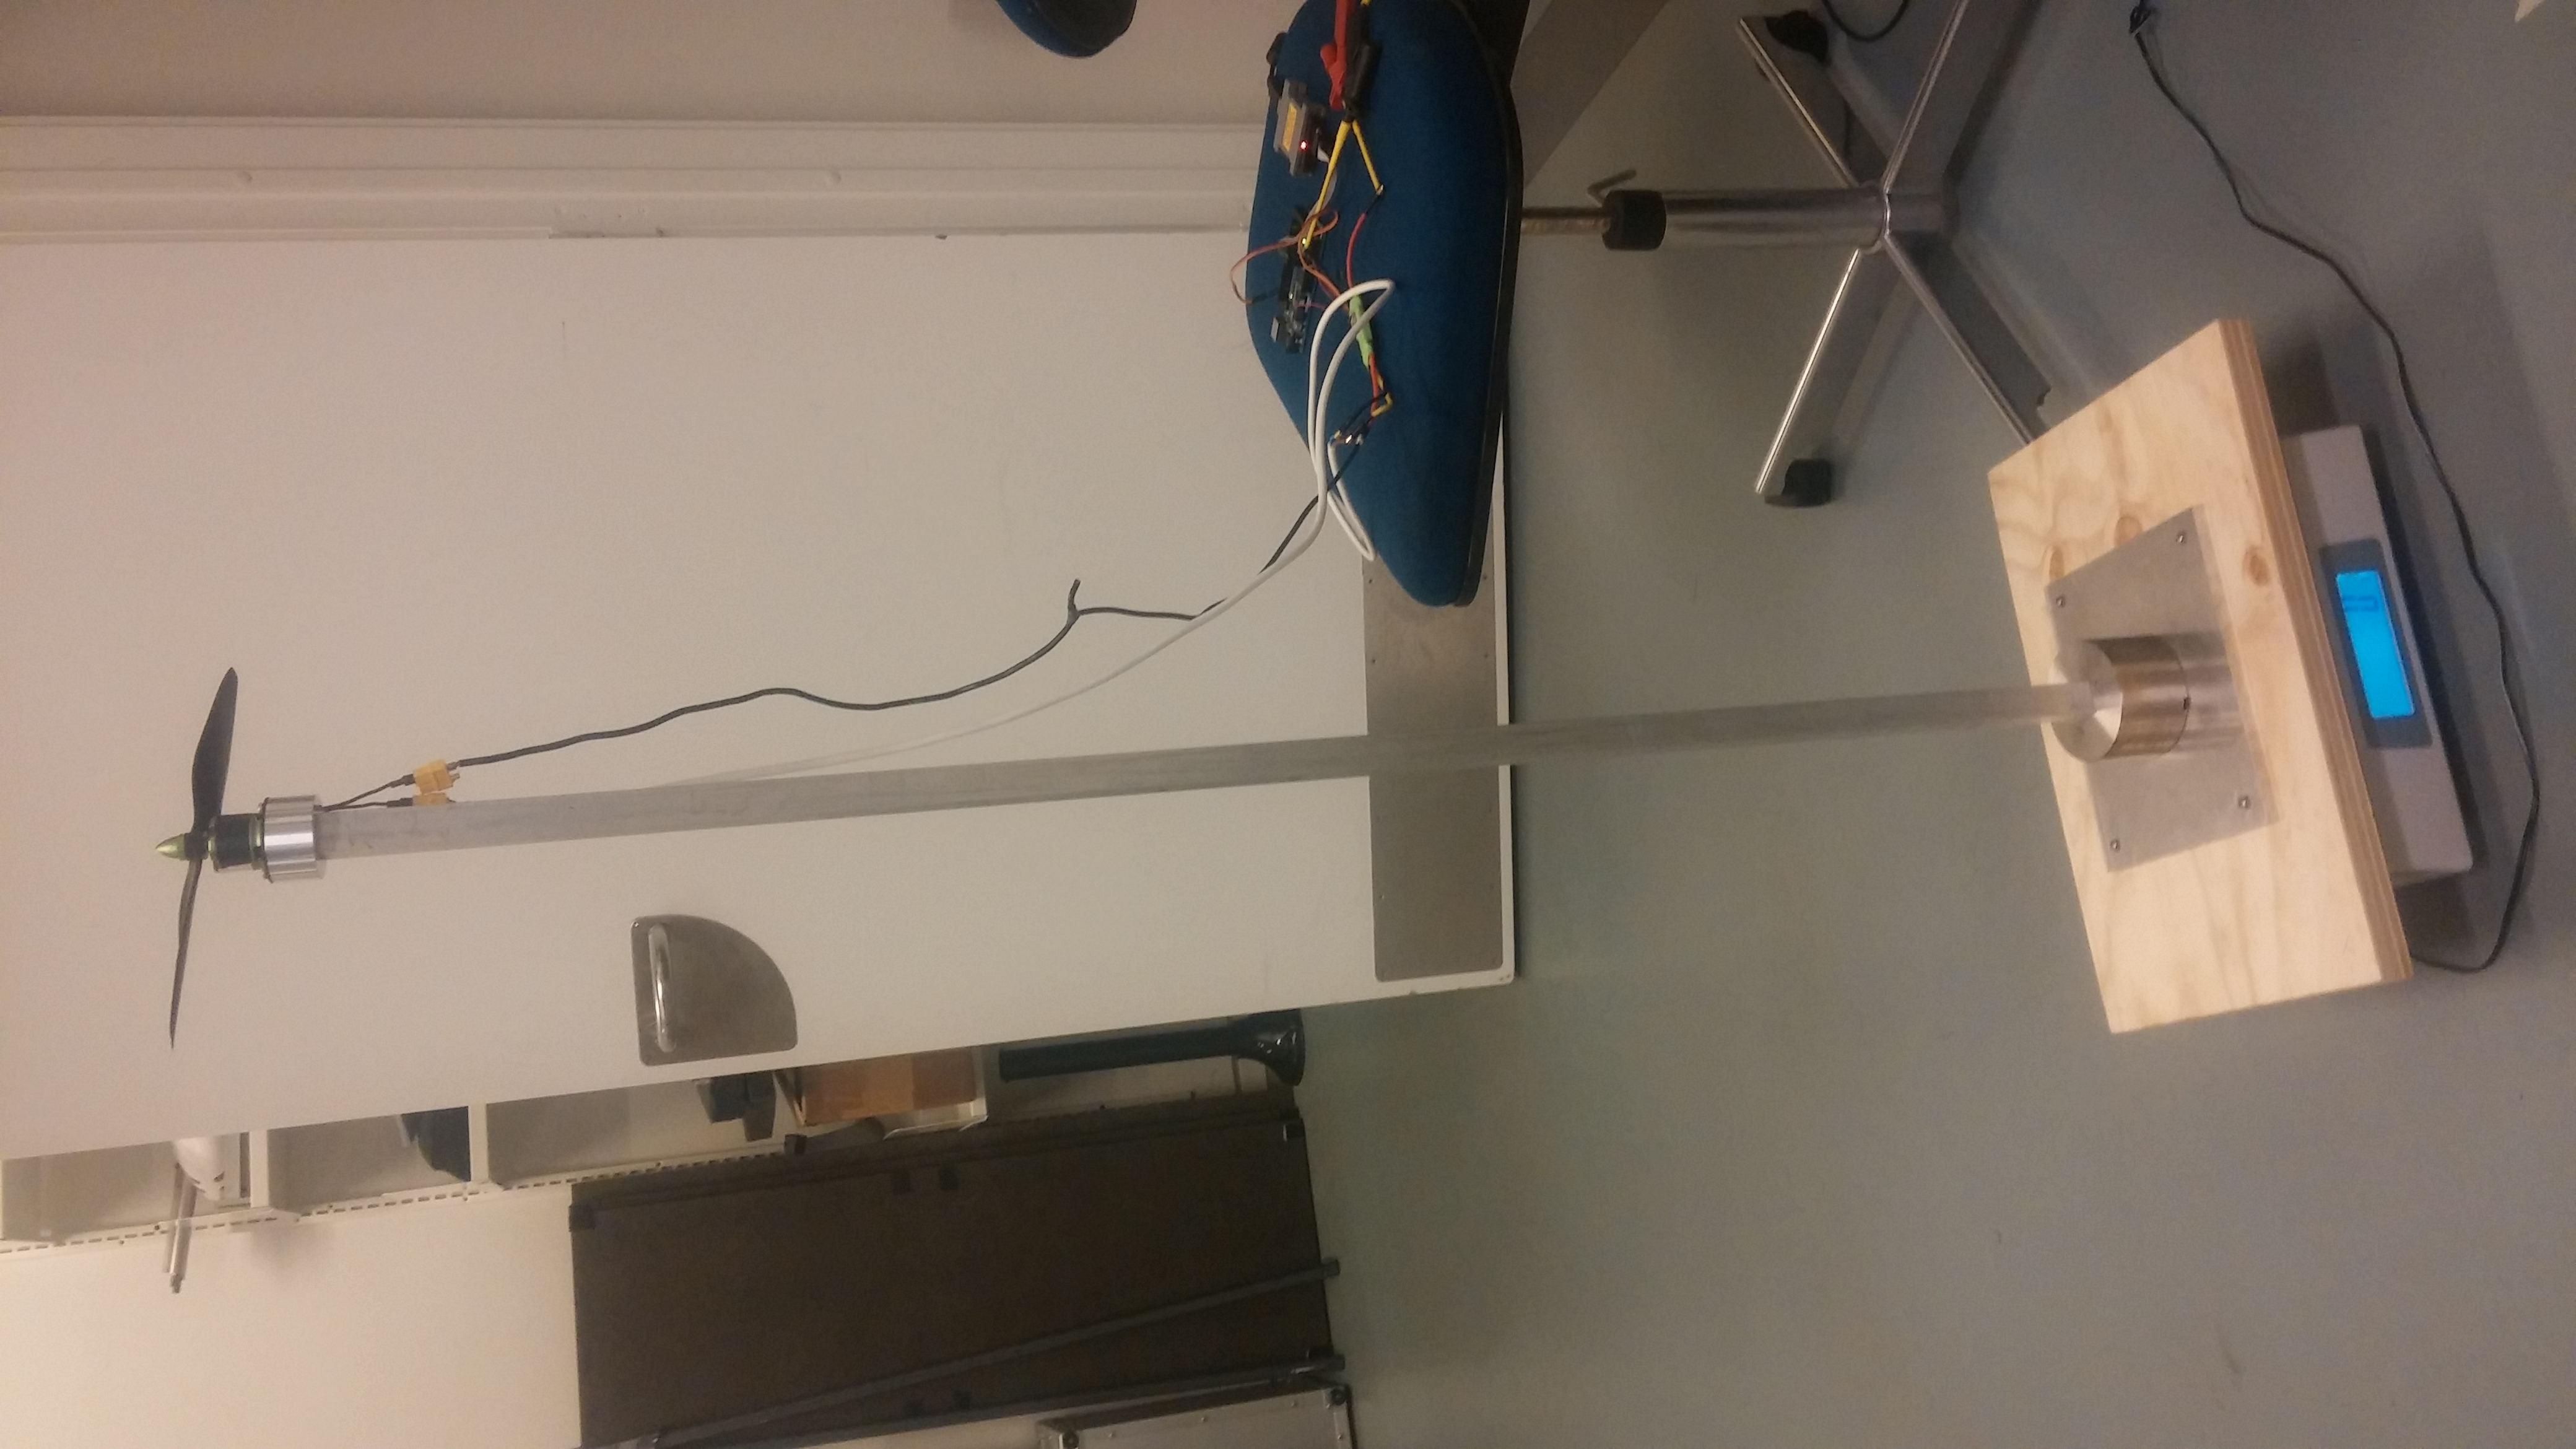
\includegraphics[scale=0.05,angle =-90]{figures/ThrustTestSetup}
%	\caption{The setup for the thrust test.}
%	\label{ThrustTest}
%\end{figure}

\subsubsection{List of Equipment}
\begin{table}[H]
	\begin{tabular}{|l|l|p{4.3cm}|}
		\hline%------------------------------------------------------------------------------------------------------------
		\textbf{Instrument}                          &  \textbf{AAU-no.}  &  \textbf{Type}                       \\
		\hline%------------------------------------------------------------------------------------------------------------
		Tachometer                                   &  08246             &  Shimpo DT-205		                   \\
		\hline%------------------------------------------------------------------------------------------------------------
	    Power Supply (11.1 V)                        &  64565             &  ES 030-5                 \\
		\hline%------------------------------------------------------------------------------------------------------------
		Processing Unit                              &  N/A               & Arduino Mega 2560    \\
		\hline%------------------------------------------------------------------------------------------------------------
		Motor                                        &  N/A               & Multistar 2213-935     \\
		\hline%------------------------------------------------------------------------------------------------------------
		Motor Speed Controller                       &  N/A               &  -      \\
		\hline%------------------------------------------------------------------------------------------------------------
		Propeller                                    &  N/A               & Turnigy 1045R     \\
		\hline%------------------------------------------------------------------------------------------------------------	
	\end{tabular}
\end{table}

\subsubsection{Procedure}
\begin{enumerate}
	\item Connect the power supply to the motor controller and the Arduino Mega to the computer though the programmer. One PWM pin and GND pin from the board must be connected to the driver signal cables yellow and brown respectively. 
	\item Run the program with a fixed PWM duty for each test.
	\item Wait for the speed to stabilize and measure it with the tachometer. 
	\item Repeat with a different duty cycle.
\end{enumerate}

\subsubsection{Results}
\begin{table}[H]
	\centering
	\begin{tabular}{|l|l|l|l|p{4.3cm}|}
		\hline%------------------------------------------------------------------------------------------------------------
		\textbf{Duty Cycle}    & \textbf{Motor Speed [rpm]} & \textbf{Motor Speed [rad/s]} \\ 
		\hline%------------------------------------------------------------------------------------------------------------
		9.4                & 1393         	   &  145.87                                       \\
		\hline%------------------------------------------------------------------------------------------------------------
		 9.5      &  2111 						       &  221.06				                \\
		\hline%------------------------------------------------------------------------------------------------------------
		 9.6       &  2335                               &  244.52   			                  \\
		\hline%------------------------------------------------------------------------------------------------------------
		9.7    & 2774                               &  290.49  			                       \\
		\hline%------------------------------------------------------------------------------------------------------------
		10   &    2868                               &  300.34                                 \\
		\hline%------------------------------------------------------------------------------------------------------------
		10.2   &  2930 						       &  306.83				                   \\
		\hline%------------------------------------------------------------------------------------------------------------
		10.5 &  3303                               &  317.62    			                    \\
		\hline%------------------------------------------------------------------------------------------------------------
		 10.8   &    3105                               &  325.15                               \\
		\hline%------------------------------------------------------------------------------------------------------------
		11.1     &  3185 						       &  333.53				                \\
		\hline%------------------------------------------------------------------------------------------------------------
	\end{tabular}
	\caption{Results obtained when applying a duty cycle of 170 to 256 in the motor speed reference.}
\end{table}

\fxnote{Put final numbers}